\section{Bestimmung des Ziels der Aufmerksamkeit}
\label{calc_Position}
Um das Ziel der Aufmerksamkeit einer Person zu bestimmen, muss die reale Position ermittelt werden. Die Orientierung des Gesichtes und die Blickrichtung können als Verlauf einer Ursprungsgerade betrachtet werden, mit dem Ursprung an der Position des Gesichtes im Raum.\\
Ist der Ursprung und die Gerade bekannt, so kann ermittelt werden, ob sie durch bestimmte Punkte im Raum verläuft. Ist dies der Fall, so wird dieser Punkt wahrscheinlich betrachtet und ist Ziel der Aufmerksamkeit der Person.
\subsection{Bestimmung der Position \& Orientierung des Gesichts}
Wird ein weiter entfernterer Punkt von beiden Augen fokussiert, so kann die Blickrichtung beider Augen als parallel angenommen werden, da der unterschied zwischen Beiden minimal ausfällt. Um den Fehler zu minimieren wird als Ergebnis die durchschnittliche Blickrichtung beider Augen verwendet. Da die Berechnung für jedes Auge unabhängig vom anderen ausgeführt, wodurch Messungenauigkeiten dazu führen, das die berechnete Blickrichtung der beiden Augen in verschiedene Richtung verlaufen\\
Zur Bestimmung der Translation und Orientierung des Gesichtes wird ein CLNF bzw. PDM eingesetzt. Dabei wurde es mit der Kameraabbildung von 3D-Landmarks eines normierten Kopfes in verschiedenen Ausrichtungen initialisiert. Das normierte Ergebnis kann mit den passenden Kameraparameter von der Aufnahme angepasst werden um die reale Position und Orientierung zu bestimmen.
\subsubsection{Abschätzen der Kameraparameter}
Sind keine Kameraparameter bekannt, so können diese anhand der Bildauflösung grob geschätzt werden. Bei der Schätzung der Brennweite für ein Bild mit einer Dimension $I_x\times I_y$ wird das Standardobjektiv mit einer Auflösung von $640 \times 480$ Pixel angenommen, somit ergebenen sich die Brennweiten $f_x$ und $f_y$ wie folgt:
\begin{align*}
f_x = 500\cdot \frac{I_x}{640}\\
f_y = 500\cdot \frac{I_y}{480}
\end{align*}
\subsubsection{Position \& Orientierung}
\label{OpenFace_Pos_Ori}
Zur Bestimmung der Kopfposition $P= \begin{pmatrix}
X_{avg} & Y_{avg} & Z_{avg}
\end{pmatrix}^t$ im Kamerakoordinaten wird die Größe, ein Skalierungsfaktor der normierten Kopfgröße $S_G$, im Bild verwendet.\\
Bei der Abbildung von Welt- nach Bild-Koordinaten gilt: $x=f\cdot \frac{X}{Z}$ und $ y=f\cdot \frac{Y}{Z}$, damit kann die Tiefe wie folgt abgeschätzt werden.\\
Sei $P_1 = \begin{pmatrix}
X_1&Y_1&Z_1
\end{pmatrix}^t, P_2= \begin{pmatrix}
X_2&Y_2&Z_2
\end{pmatrix}$ die Beschreibung der Größe $G$ eines Kopfes mit:\\
\begin{align*}
a &= \frac{\sqrt{(X_1-X_2)^2+(Y_1+Y_2)^2}}{\frac{Z_1-Z_2}{2}} =\frac{G}{Z_{avg}}\\
S &= \frac{S_G}{G}\\
\Rightarrow a\cdot f &= f\cdot\frac{G}{Z_{avg}} = S_G\\
Z_{avg} &= \frac{f}{S_G}\cdot G = \frac{f}{S}\\
X_{avg} &= \frac{x \cdot Z_{avg}}{f}\\
Y_{avg} &= \frac{y \cdot Z_{avg}}{f}\\
\end{align*}
Dies beschreibt allerdings nur eine Annäherung an die tatsächliche Position, da die Distanz mit Hilfe einer durchschnittlichen Kopfgröße geschätzt wird.\\
\cite{OpenFace}
\subsubsection{Bestimmung der Blickrichtung}
\label{OpenFace_Blickrichtung}
Für möglichst genaue Ergebnisse wird für die Augenpartie ein weiteres CNN eingesetzt das nur auf diesem Bildaufschnitt arbeitet und weitere 28 Landmarks bestimmt. Durch diese werden die Lider, Iris und Pupille dargestellt und für jedes Auge separat bestimmt.\\
Zur Bestimmung der Blickrichtung wird wie folgt vorgegangen: Zuerst wird der Strahl bestimmt der, ausgehend vom Zentrum der Kamera, durch das Zentrum der Pupille verläuft. Nun wir der Schnittpunkt zwischen diesem Strahl und einer Sphäre bestimmt, die das Auge repräsentiert. Anschließend wird ein Strahl bestimmt der vom Zentrum der Sphäre ausgehend durch den berechneten Schnittpunkt verläuft, dies ist die resultierende Blickrichtung.
\subsubsection{Zusammenhang von Bildposition \& Weltposition}
Als Ausgangspunkt werden die Ergebnisse des CNN verwendet um die Position zu bestimmen. Zur Bestimmung der Orientierung $R$ liefert auch das CNN ein Ergebnis $R_{CNN}$. Allerdings stimmt es nur im Zentrum des Bildes, da am Rand immer mehr die Orientierung der einzelnen Pixel mit berücksichtigt werden muss.\\
\begin{align*}
euler_x &= \tan^{-1}(\frac{\sqrt{X^2+Z^2}}{Z^2})\\
euler_y &= \tan^{-1}(\frac{\sqrt{Y^2+Z^2}}{Z^2})\\
R_{pos} &= R(euler_x,euler_y,0)\text{ Umwandlung zur Rotationsmatrix}\\
R &= R_{CNN}\cdot R{pos}
\end{align*}
Eine weitere Verbesserung kann erreicht werden, indem die gefunden 2D-Landmarks mit Hilfe des PDM in 3D zu überführen. Um anschließend die Überführung von 2D nach 3D-Koordinaten erneut zu bestimmen um die Orientierung und Position zu ermitteln. Auch bei diesem Verfahren muss die Pixelorientierung beachtete werden. Allerdings ist auch ein Tiefendbild nötig, da ansonsten die Fehler weiter verstärkt werden. Daher ist es in der aktuellen Anwendung nicht sinnvoll einsetzbar.
\subsection{Größe und Genauigkeit}
Um die Qualität der Berechnung auf verschiedenen Distanzen zu ermitteln, wurde der Datensatz Forests for Real Time 3D Face Analysis \cite{database_Face_Ori} verwendet, da für jedes Gesicht die Position und Orientierung bekannt ist.
Die durchschnittliche Distanz zwischen Kamera und Kopf beträgt ca $70cm$ bei einer Kopfbreite von 78 Pixel. Um die verschiedenen Distanzen zwischen Probanden und Kamera zu simulieren, wurden die Bilder mit dem angegebene Skalierungsfaktor (X-Achse) linear verkleinert.\\
Da verschiedene Verfahren zur Bestimmung der Position und Orientierung zur Verfügung stehen, sollen diese miteinander verglichen werden. Zur Bestimmung wurde nur das RGB-Bild verwendet und nicht zusätzlich die Tiefeinaufnahme, da dies in der Anwendung auch nicht vorhanden sind.
\subsubsection{Position}
Zur Bestimmung der Position gibt es zwei Verfahren, die direkte mittels Brennweite und Skalierung oder Überführungsmatrix von 3D zu 2D Landmarks arbeiten.\\
Die Funktionen PoseCamera und PoseWorld verwenden die einfache Bestimmung mittels Skalierung und CorrectPoseCamera und CorrectPoseWorld die Überführung von 3D und 2D Landmarks, daher überlagern sich die Linien in \autoref{img_Verfahren_Pos}, da die jeweiligen Verfahren nach dem selben Prinzip rechnen.\\
Der schnelle Abfall der Genauigkeit bei der Skalierung $0,25$ ist an der selben Stelle an der auch die Detektionsrate stark absinkt, siehe \autoref{OpenFace_skal}. Somit kann das Verfahren bis zu seiner Grenze eingesetzt werden und erst, wenn die Detektion schwierig wird steigt auch der Fehler.
\begin{figure}
	\centering
	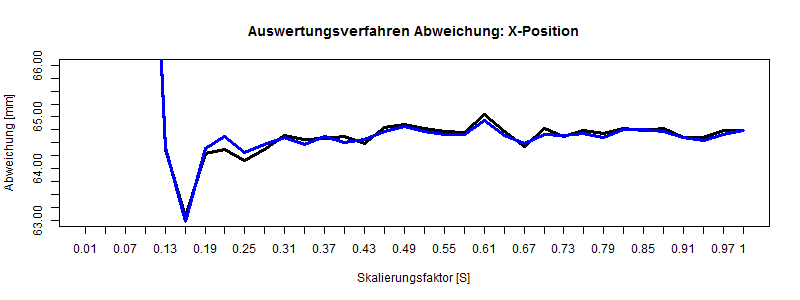
\includegraphics[width=\linewidth]{img_Skalierung/Verfahren_TX}
	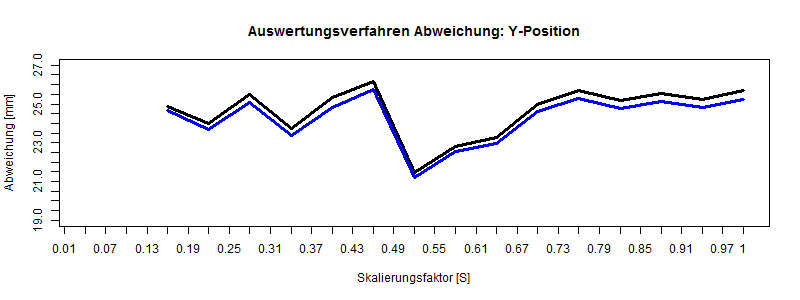
\includegraphics[width=\linewidth]{img_Skalierung/Verfahren_TY}
	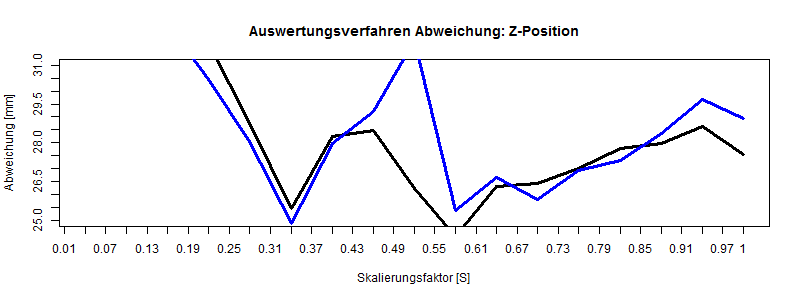
\includegraphics[width=\linewidth]{img_Skalierung/Verfahren_TZ}
	\caption{Dargestellt ist der Median der Abweichung in Millimeter der Positionsbestimmung auf Bilder die mit Lanczos skaliert wurden.\\
	PoseWorld (schwarz), PoseCamera (rot), CorrectPoseCamera (grün) und PoseWorld (blau)\\
	Oben: X-Position, Mitte: Y-Position, Unten: Z-Position}
	\label{img_Verfahren_Pos}
\end{figure}
\subsubsection{Orientierung}
Bei der Rotation Zeigen sich nun Unterscheiden zwischen den einzelnen Verfahren, da bei PoseWorld und CorrectPoseWorld auch die Position im Kamerabild berücksichtigt wird.\\
Es Zeigt sich in \autoref{img_Verfahren_Rot}, das die zusätzliche Korrektur das Ergebnis weiter verbessern, vor allem wenn sich das Gesicht weit außerhalb des Zentrums befindet.
\begin{figure}
	\centering
	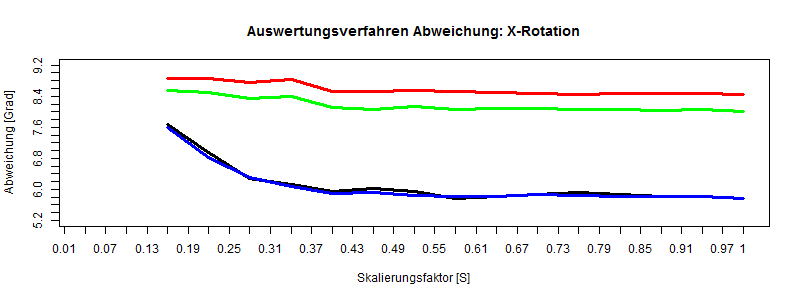
\includegraphics[width=\linewidth]{img_Skalierung/Verfahren_RX}
	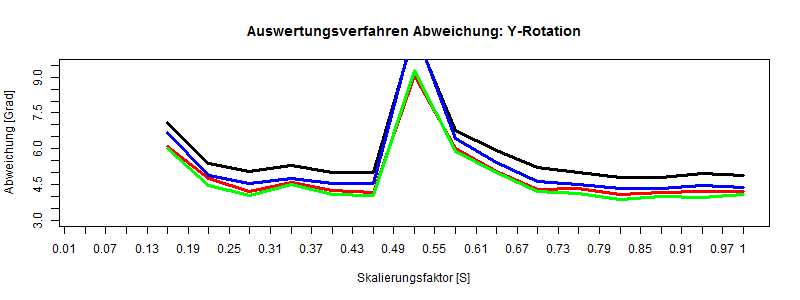
\includegraphics[width=\linewidth]{img_Skalierung/Verfahren_RY}
	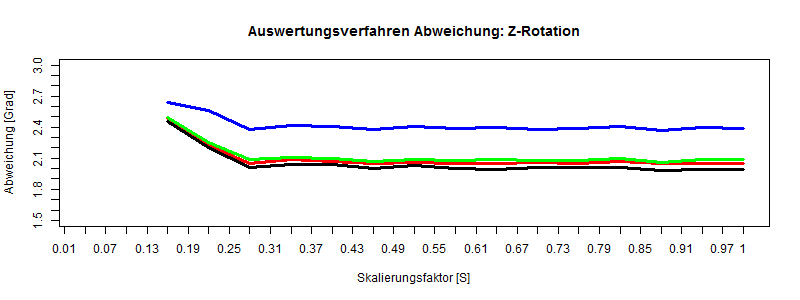
\includegraphics[width=\linewidth]{img_Skalierung/Verfahren_RZ}
	\caption{Dargestellt ist der Median der Abweichung in Grad der Positionsbestimmung auf Bilder die mit Lanczos skaliert wurden.\\
		PoseWorld (schwarz), PoseCamera (rot), CorrectPoseCamera (grün) und CorrectPoseWorld (blau)\\
		Oben: X-Rotation, Mitte: Y-Rotation, Unten: Z-Rotation}
	\label{img_Verfahren_Rot}
\end{figure}
\subsubsection{Ergebnis}
Es zeigt sich, dass CorrectPoseWorld, also die komplexe Bestimmung der Position mittels 2D/3D Landmarks und zusätzlicher Korrektur der Winkel die besten Ergebnisse liefert im Test.\\
Im Test ist die Überführung von 3D ud 2D Landmarks am besten (CorrectPoseCamera und CorrectPoseWorld) kann sich allerdings auch ändern wenn die Kamera Parameter besser abgeschätzt sind, da ohne eine Tiefenaufnahme die korrekte Überführung nur geschätzt werden kann und sich Fehler fortpflanzen können.
\subsection{Bestimmung eines Punktes, auf der die Aufmerksamkeit liegt}
Von Interesse ist vor allem der Punkt auf den der Blick ruht bzw. das Gesicht ausgerichtet ist.\\
Bestimmung des Richtungsvektors $V$ aus der Rotationsmatrix
\[V= R\cdot (0,0,-1)^T\] 
Aus der Blickrichtung mehrerer Probanden kann auch der reale Punkt der Aufmerksamkeit ermittelt werden. Dazu wird die Blickrichtung als Linie $L_i = s \cdot n_i+ p_i$ beschrieben mit $s\in \mathbb{R}$ und $n_i,p_i \in \mathbb{R}^3$ verwendet.
\begin{align*}
c&=(\sum_{i} I -n_in_i^T)^{-1}
(\sum_{i} (I -n_in_i^T)\cdot p_i)
\end{align*}
Bei Verwendung der Gesichtsorientierung ergibt sich das Problem den konkreten Blickpunkt zu ermitteln, da die Augenbewegung nicht erfasst werden kann.
So muss ein Kegel, der den üblichen Bereich der Augenbewegung umfasst, um die Orientierung berücksichtigt werden als Fehlertoleranz und der gesamte Bereich kommt als Lösungen in Frage.
Außerdem liegt der Punkt der Aufmerksamkeit meist außerhalb des Bildbereiches der Kamera und muss entsprechend von einer Anwendung interpretiert werden.\\
Soll die Position des Ziels auf nahezu parallel verlaufende oder stark verrausche Ergebnisse berechnet werden, so ist die Bestimmung des Schnittpunkts nach dem obigen Verfahren nicht möglich.\\
Eine einfache Variante ist das Verwenden des durchschnittlichen Richtungsvektors $V_{avg}$ und Position $P_{avg}$ der Probanden. Die Tiefe $a$ muss nun geschätzt werden um das Ziel $P=V\cdot a$ zu bestimmen.